\chapter{Approach}
\label{ch:approach}
\graphicspath{{image_directory/approach/}}

	The LWR equation (\ref{eq:LWR}) is already presented in conservative form as a hyperbolic PDE \cite{Toro09}. The following present this in the framework of Euler gas dynamics equations governing this compressible flow,
	\begin{equation}
		\frac{\partial\mathbf{U}}{\partial t}+\frac{\partial\mathbf{F}(\mathbf{U})}{\partial x}=0, 
		\quad
		with
		\quad
		\mathbf{U}=\left[\rho\right], 
		\quad and \quad
		\mathbf{F}=\left[\rho u\right],		
		\label{eq:euler}
	\end{equation}
	where $\mathbf{U}$ represents the conserved density $\rho$. In the program code, the conserved state, $\mathbf{U}$, are known and are used with the fundamental flow relationship to calculate the flux, $\mathbf{F}$, hence $\mathbf{F}=\mathbf{F}(\mathbf{U})$. From this formulation, if $\mathbf{U}$ is discretised over the current time, $n$, and the next time step $n+1$, and $\mathbf{F}$ over left and right cell interfaces, $\mathbf{F}_{i-1/2}$ and $\mathbf{F}_{i+1/2}$ respectively, then an update scheme is
	\begin{equation}
		\mathbf{U}_i^{n+1}=\mathbf{U}_i^n-\frac{\Delta t}{\Delta x}\left(\mathbf{F}_{i+1/2}-\mathbf{F}_{i-1/2}\right).\nonumber
	\end{equation}
	The values of $\mathbf{F}_{i+1/2}-\mathbf{F}_{i-1/2}$ introduce a difficulty, finite difference approximations construct a piecewise continuous solution profile as shown in Figure \ref{fig:1d_discretisation}, so interface values are discontinuous and need alternative treatment. To solve $\mathbf{U}$ over cell interface discontinuities, the local Riemann problem is constructed for Equation \ref{eq:euler} with the initial conditions
	\begin{equation}
		\mathbf{U}(x,t=0)=
		\begin{cases}
			\mathbf{U}_L, & if \quad x<0,\\
			\mathbf{U}_R, & if \quad x>0,
		\end{cases}
		\label{eq:init_con}
	\end{equation}
	where the variables $x$ and $t$ are mapped in the following way
	\begin{equation}
		(x_{i-1/2},x_{i+1/2})\mapsto(-\Delta x/2,\Delta x/2), 
		\quad
		and
		\quad
		(t_n,t_{n+1})\mapsto(0,\Delta t).
		\label{eq:local_scale}
	\end{equation}
	The following sections discuss more numerical approaches and some Riemann solving methods for the problem in Equations \ref{eq:euler} and \ref{eq:init_con}. This governing formulation is shown in more detail in \cite{Chung02},\cite{Toro09},\cite{Toro94}, while many of the following details can be found in \cite{TakisNotes}.
	\begin{figure}
    		\centering
        		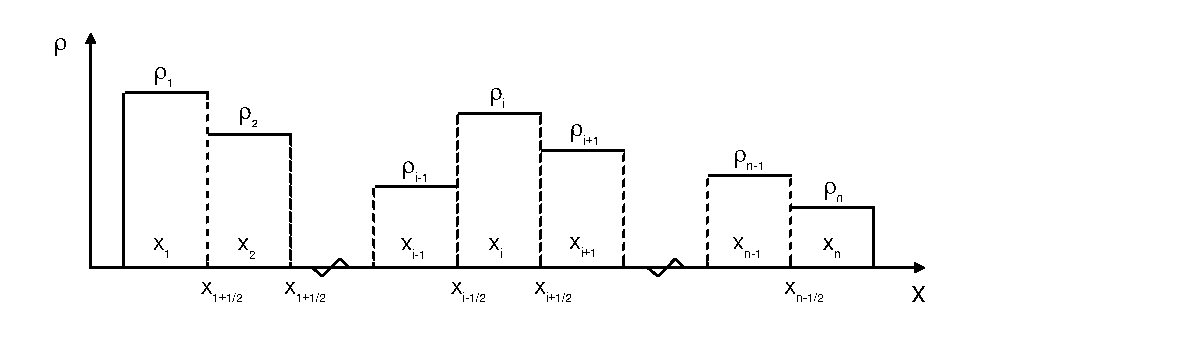
\includegraphics[trim=20 20 120 10,clip,width=\textwidth]{discretisation.pdf}
		\caption[Approach : 1D finite difference discretisation]{Discretisation of a 1D spatial domain for a single time. For $i\in\mathds{Z}$, $x_i$ represent the control volumes where single Godunov averaged solutions are stored, $\rho_i$. The cell interfaces are represented at locations $x_{i\pm1/2}$; as single solutions are stored in one cell, there are discontinuities at each cell interface location.}
		\label{fig:1d_discretisation}
	\end{figure}
	
\section{Compressible Flow Waves}
\label{sec:waves}

	Compressible dynamics numerical methods have been developed to allow flow variables to exhibit discontinuous derivatives in space, these variable jumps are due to the presence of flow waves. There are four types of compressible waves discussed here; normal shock, contact surface, rarefaction, and compression waves. When a region of high pressure and density is separated by a diaphragm from a region of low pressure and density\footnote{Such as the initial conditions for 1D shock tube and 2D explosion case.}, some of these waves occur. \\ \\
	Normal shock waves, such as the shock present on the upper surface of a transonic aerofoil, are normal to a surface. Contact surfaces propagate through a dynamic fluid as the discontinuous interface between two materials. Rarefaction waves represent gradual longitudinal expansion, propagating through the flow. Compression is the opposite of rarefaction, where a compression of characteristics move with the flow.
	
	
\section{Godunov-Type Methods}
\label{sec:Godunov}

	The Godunov method assumes piecewise constant solution profiles (see Figure \ref{fig:1d_discretisation}), with discontinuities along cell interfaces that induce many local Riemann problems \cite{Toro09}. Godunov's method improves on central-based schemes by having the capability to distinguish between compression and expansion fan waves \cite{Jayanti18}. Godunov \cite{Godunov59} suggested the following method for computing the interface flux approximations:
	\begin{itemize}
	\item[1.] Construct two \emph{local} Riemann problems over a data pairs $(\rho_{i-1}^n,\rho_{i}^n)$ and $(\rho_i^n,\rho_{i+1}^n)$,
	\item[2.] Average the two solutions over $[x_{i-1/2},x_{i+1/2}]$,
	\item[3.] Assign a value for $\rho_i^{n+1}$,
	\item[4.] Then the Godunov flux is approximated by
		      \begin{equation}
		      	\mathbf{F}_{i\pm1/2}=\mathbf{F}\left(\mathbf{U}_{i\pm1/2}\right). \nonumber
		      \end{equation}
	\end{itemize}
	The two Riemann problems are formulated locally (by scaling the variables as in Equation \ref{eq:local_scale}) with the equation $\rho_t+f(\rho)_x=0$, and each set of boundary conditions
	\begin{equation}
		(\rho_{i-1}^n,\rho_{i}^n) \, : \quad \rho(x,0)=
		\begin{cases}
			\rho_{i-1}^n, & if \quad x<0, \\
			\rho_i^n, & if \quad x>0,
		\end{cases}
		\nonumber
	\end{equation}
	\begin{equation}
		(\rho_i^n,\rho_{i+1}^n) \, : \quad \rho(x,0)=
		\begin{cases}
			\rho_i^n, & if \quad x<0, \\
			\rho_{i+1}^n, & if \quad x>0.
		\end{cases}
		\nonumber
	\end{equation}
	The cell averaging for $\rho_i^{n+1}$ is taken over the cell width, however with the locally formulated Riemann problems this is over $[-\Delta x/2,\Delta x/2]$, for the two Riemann problem solutions $\tilde \rho_{i-1/2}$ and $\tilde \rho_{i+1/2}$. The new solution is given by
	\begin{equation}
		\Delta x\cdot \rho_i^{n+1}=\int_{-\Delta x/2}^0\tilde \rho_{i-1/2}\mathrm{d}x +\int_0^{\Delta x/2}\tilde \rho_{i+1/2}\mathrm{d}x\label{eq:GodunovUpdate}
	\end{equation}
	Fluid dynamics problems are usually formulated as a combination of varying PDEs, solutions to which are highly sensitive to numerical methods \cite{Chung02}. Godunov schemes are useful when applied to hyperbolic systems, however have limitations for other types of PDEs. Elliptical problems have no real characteristic curves so flow variable derivatives are smooth with no discontinuities, hence the Godunov method and local Riemann problems are not useful \cite{Chung02}. The major disadvantage of using Godunov schemes with Riemann solvers for shock capturing flow is the extra computational cost over a second order scheme with artificial viscosity \cite{Woodward84}. Riemann solvers become complicated to implement if an equation of state cannot be represented with a gamma law. Analytical solutions of Riemann problems exist for the Euler equations however are computationally expensive, hence the Godunov local Riemann problems are solved using approximate methods shown in Section \ref{sec:RSFC}.	

\section{Approximate Riemann Solvers}
\label{sec:RSFC}

	The following methods for finding approximate solutions to local Riemann problems at each cell interface are presented for interest, only the Lax-Friedrichs, Rusanov, HLL and Murman-Roe solvers are included in the TFM program code, see Appendix \ref{code:main} lines [394-470]. As shown in Chapter \ref{ch:randd}, one of the flaws of this model is the ill defined Riemann solvers. An appropriate definition of parameters involved in the following methods is needed to yield a more realistic solution to the cell interfaces. This process in the simulation is known both as the approximate local Riemann problem solution and the calculation of numerical fluxes. These local problems are too computationally costly to apply exact Riemann solvers, hence approximate methods are used to cut this cost \cite{Laney98}.
	
\subsection{Rusanov and Lax-Friedrichs Flux}
\label{sec:RLF}

	The Rusanov \cite{Rusanov61} and Lax-Friedrichs \cite{Lax54} fluxes can both be written in the form
	\begin{equation}
		\mathbf{F}=\frac{1}{2}\left[\left(\mathbf{F}_L+\mathbf{F}_R\right)-S^+\left(\mathbf{U}_R-\mathbf{U}_L\right)\right], \label{eq:Rusanov}
	\end{equation}
	where the wave speed $S^+$ is calculated from local data in the Riemann problem, where both
	\begin{equation}
		S^+=\max\left(\left|f'\left(u_L\right)\right|,\left|f'\left(u_R\right)\right|\right),\label{eq:srus}
	\end{equation}
	\begin{equation}
		S^+=\frac{\Delta x}{\Delta t},\label{eq:slf}
	\end{equation}
	represent the maximum wave speed for the Rusanov (Equation \ref{eq:srus}) and Lax-Friedrichs (Equation \ref{eq:slf}) fluxes. These solvers can be found in Appendix \ref{code:main} lines [412-430], where the left and right state derivatives (Rusanov) are calculated from the chosen stream model. 
	
\subsection{Murman-Roe}
\label{sec:MR}

	The popular Roe solver defined for a scalar system is named the Murman-Roe solver \cite{Murman74}. Murman defines the wave velocity $a$ as the Rankine-Hugoniot velocity, 
	\begin{equation}
		a\left(\rho_L,\rho_R\right)=\frac{f_L-f_R}{\rho_L-\rho_R},
	\end{equation}
	and flux,
	\begin{equation}
		f\left(\rho_{L},\rho_{R}\right)=\frac{1}{2}\left(f_{L}+f_{R}\right)-\left|a\left(\rho_L,\rho_R\right)\right|\left(\rho_{R}-\rho_{L}\right),
	\end{equation} 
	if $\rho_L\neq\rho_R$.  However if $\rho_L=\rho_R$ then the velocity is defined as,
	\begin{equation}
		a\left(\rho_L,\rho_R\right)=f'_L=f'_R,
	\end{equation}
	and the flux depends on this velocity as follows,
	\begin{equation}
		f\left(\rho_{L},\rho_{R}\right)=
			\begin{cases}
				f_L, &\text{if}\quad a\left(\rho_L,\rho_R\right)>0,\\
				f_R, &\text{if}\quad a\left(\rho_L,\rho_R\right)\leq0.
			\end{cases}
	\end{equation}

\subsection{HLL}
\label{sec:HLL}

	Harten, Lax and van Leer \cite{HLL83} suggested a Riemann solver which assumes a wave formation of two waves, however this is incorrect for the Euler equations and only holds for two equation hyperbolic systems \cite{Toro09}. Hence the integral-form conservation equations are split over three regions, left and right states and a single \emph{star} region. Depending on the choice of left and right wave speed values, $S_L$ and $S_R$, the HLL flux is given by
	\begin{equation}
		\mathbf{F}=
		\begin{cases}
			\mathbf{F}_L, & if \quad 0\leq S_L, \\
			\mathbf{F}_M=\frac{S_R\mathbf{F}_L-S_L\mathbf{F}_R+S_LS_R\left(\mathbf{U}_R-\mathbf{U}_L\right)}{S_R-S_L}, & if \quad S_L\leq0\leq S_R,\\
			\mathbf{F}_R, & if \quad S_R\leq0.
		\end{cases}
		\nonumber
	\end{equation}
	As well as this formulation, Toro et al. \cite{Toro94} outline the problem with this Riemann solver. Namely the difficulty in finding reliable and simple estimates for the left and right wave speeds. Toro developed the HLL solver further, details of the HLLC Riemann solver are given in Appendix \ref{ap:HLLCriemann}. 
	
\subsection{Wave Speed Estimations}
	All previous Riemann solvers have depended on a set of parameters defining the behaviour of each Riemann solver, including the wave speed values of $S_L,\,S_R,\,S_*$. Davis \cite{Davis88} suggested a set of simple estimates for Riemann solvers in compressible gas dynamics where the quantity $a$ represents the local speed of sound. Toro showed that these estimates are however impractical for computations \cite{Toro09},
	\begin{equation}
		S_L=u_L-a_L, \quad S_R=u_R+a_R, \nonumber
	\end{equation}
	and
	\begin{equation}
		S_L=\min\left(u_L-a_L,u_R-a_R\right), \quad S_R=\max\left(u_L+a_L,u_R+a_R\right). \nonumber
	\end{equation}
	Davis \cite{Davis88} also uses the Roe-averaged eigenvalues
	\begin{equation}
		S_L=\tilde u-\tilde a, \quad and \quad S_R=\tilde u+\tilde a, \nonumber
	\end{equation}
	with Roe-averaged speeds denoted by $\sim$, which lead to a much more effective scheme. Davis also recognised how the Rusanov flux (Equation \ref{eq:Rusanov}) can be recovered from the HLL formulation by setting $S_L=-S^+$ and $S_R=S^+$ for some choice of $S^+$ mentioned in Section \ref{sec:RLF}. This aspect of the relationship between solving local Riemann problems in cell reconstruction in TFM is not equivalent to other fields such as gas dynamics, appropriate parameters to describe the local Riemann problems need to be established for the solvers described here to be most effective.
	
\section{Spatial Reconstruction}

	Prior to providing left and right states to a chosen Riemann solver to evaluate the numerical flux and proceed with the iteration, one can reconstruct the cell variable value in many ways. The most simple approach is named 1$^{st}$ order as the values provided for numerical flux calculations are in fact the cell average Godunov values themselves with no reconstruction applied. The next improvement is the 2$^{nd}$ order total variation diminishing scheme. At each cell interface (cell $i$, left $i-1/2$, right $i+1/2$), the left and right densities are 2$^{nd}$ order TVD reconstructed according to
	\begin{equation}
		\rho_L=\rho_i+\frac{\Delta_i}{2}, \quad and \quad \rho_R=\rho_{i+1}-\frac{\Delta_{i+1}}{2},\label{eq:tdv}
	\end{equation} 
	\begin{equation}
		\Delta_i=\mathrm{minmod}\left(\rho_i-\rho_{i-1},\rho_{i+1}-\rho_i\right), \nonumber
	\end{equation}
	\begin{equation}
		\mathrm{minmod}\left(x,y\right)=\frac{1}{2}\left(\mathrm{sign}\left(x\right)+\mathrm{sign}\left(y\right)\right)\min\left(\left|x\right|,\left|y\right|\right), \label{eq:minmod}
	\end{equation}
	where the slope limit $\Delta_i$ is calculated from the minmod limiter function.
	
\subsection{High Resolution Schemes}
\label{sec:HRS}
	
	High resolution numerical schemes are used when fluid problems involving shocks and discontinuities are of interest with high accuracy, high resolution methods reduce oscillations to provide monotone solutions \cite{Chung02}. Monotonicity preserving schemes are at most first order accurate according to Godunov's theory, where higher order schemes introduce oscillations around discontinuities \cite{Cockburn01}. Alternative to the uniform distribution over cells in Godunov's method, the MUSCL scheme which uses linear reconstructions of Godunov cell data. When accuracy greater than second order is required, WENO schemes provide higher accuracy. See Figure \ref{fig:high_res_schemes} for the comparison of a 1D problem solution using various discussed schemes. 
	\\ \\
	The first WENO scheme was proposed by Liu, Osher and Chan in 1994 \cite{Liu94}, a novel ENO method with a higher order reconstruction. Where the ENO method chooses the smoothest interpolating polynomial, the weighted scheme uses a convex combination of all polynomials with weights specifically chosen to improve on the accuracy of the ENO scheme. ENO schemes attempt higher order accuracy and to avoid oscillations at discontinuities \cite{Chung02}. WENO implementation can be either component-wise or characteristic wise, in terms of the cell reconstruction procedure. A review of reconstruction methods for ENO and WENO schemes are given in full detail in \cite{Shu97}. Component-wise applies scalar reconstruction procedures to each conserved vector component at each cell interface, then applies an exact or approximate Riemann solver to form the high resolution scheme. Characteristic-wise computes average state values, and the left and right Jacobian eigenvectors, then the eigenvectors are used to transform the cell variables to characteristic variables which are then reconstructed using WENO/ENO procedures. The component method is more simple to implement yet the characteristic method is more robust \cite{Shu97}. See Appendix \ref{ap:WENOreco} for the WENO algorithms used.
	\\ \\
	Proposed by Bram van Leer in 1979 \cite{vanLeer79} the MUSCL scheme was able to achieve second order accuracy and behaved at least an order of magnitude more efficient that Godunov schemes, equivalent of refining a mesh with factor two. Van Leer's MUSCL approximates the cell density distribution with polynomials of order $n\in\left\{2,3\right\}$, this alone would introduce large oscillations in the presence of shocks. To reduce oscillations and ensure the scheme is TVD, the slope limiter $\phi$ is applied at left and right states. TVD schemes reduce to first order at local extrema, and are as high order as the general scheme in smooth regions. The 2nd order MUSCL scheme approximates the cell density distribution with a linear slope, whereas the 3rd order scheme approximates with a parabolic slope from a second order interpolation. Oscillations may appear in solutions with large flow variable gradients due to a numerical procedure with no artificial dissipation \cite{Tu18}, the latter will reduce flow to a monotone solution however is inaccurate. To keep monotonicity yet eliminate the need for artificial dissipation, flux gradient limiters are used. Barth and Jesperson \cite{Barth89} suggest a slope limiter, $\phi_i$, which limits the gradient in the reconstruction
	\begin{equation}
		R_i\left(x_j-x_i\right)=\rho_i+\phi_i\nabla \rho_i\left(x_j-x_i\right), \quad with \quad \phi\in[0,1]. \nonumber
	\end{equation}
	Mathematical descriptions of two limiters have been summarised from Michalak and Ollivier-Gooch \cite{Gooch08}, where reconstruction is described with the need of gradient limiters and a useful algorithm for the Barth and Jespersen limiter is presented which can be developed into Venkatakrishnan's limiter. See Appendix \ref{ap:MUSCLreco} for the MUSCL algorithms used. 
	\begin{figure}
    		\centering
        		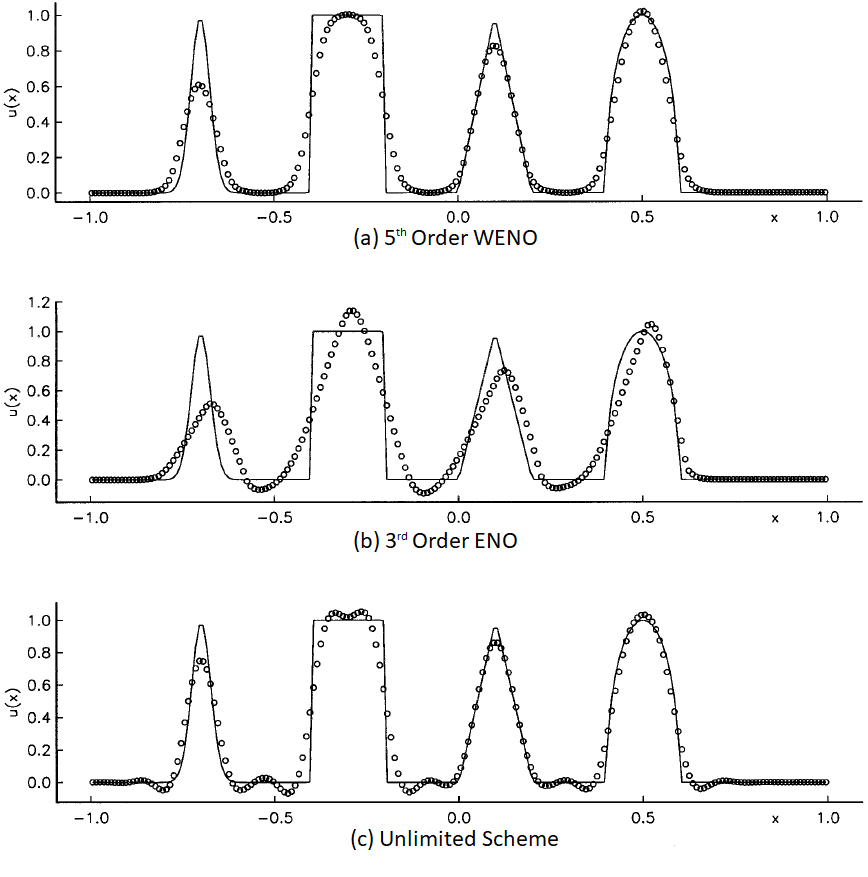
\includegraphics[trim=0 0 0 0,clip,width=0.6\textwidth]{high_res.png}
		\caption[Approach : Comparison of high resolution schemes]{1D advection equation results from Suresh and Huynh \cite{Suresh97}. The unlimited scheme (c) is not high resolution, hence oscillations appear in the solution in regions of high gradient $\partial \rho/\partial x$ discontinuities. Using the smoothest polynomial reconstruction in the 3$^{\mathrm{rd}}$-Order ENO scheme (b) finds a monotone improvement from (c). Using a specific weighted average of polynomials, the 5$^{\mathrm{rd}}$-Order WENO (a) scheme has improved accuracy by choosing appropriate polynomials not just the smoothest one, as in ENO (b). }
		\label{fig:high_res_schemes}
	\end{figure}
	
\newpage
\section{Limitations of Finite Difference Schemes}

	Finite difference is the approach of describing derivatives by finite discrete values. Chung presents many FDMs and evaluates their performance \cite{Chung02}. FDM can only be used on structured grids\footnote{More generally FDM can also be used on \emph{transformations} of orthogonal structured grids}. Hyperbolic PDEs are used to model wave propagation; FDM are limited by strict stability criterion restricting spatial and time step sizes, with are due to bounding the dissipative error growth. All \emph{implicit} FDM schemes however are unconditionally unstable. Low-resolution schemes are inaccurate at discontinuities, either over or underestimating with oscillations. Improving the order of accuracy in FDM requires more initial data. Extra solving tools are required to improve the accuracy, including high resolution methods, Riemann solvers and reconstruction procedures with gradient limiters. The higher resolution group of TDV methods are considered higher order but the accuracy is not uniform, TDV schemes may range from first to second order accuracy in different solution regions. Solving systems of hyperbolic PDEs includes the calculations of Jacobians which are computationally inconvenient. 
	
\section{Time-Update Scheme}
\label{sec:timeupdatescheme}

	The single step discretisation update given in Equation \ref{eq:GodunovUpdate} will not allow some of the higher resolution schemes to exhibit their advantages over lower resolution methods. A commonly used time-update scheme is the classical 4$^{th}$ order Runge-Kutta process. First proposed by Runge \cite{Runge1895} and further developed or finalised into a family of methods by Kutta \cite{Kutta1901}, used by many in a wide field of study the modern Runge-Kutta framework provides a strong foundation for building a sophisticated time update scheme. The classical fourth order update is used in this TFM program, and can be found in lines [552-584] of the code in Appendix \ref{code:main}. This method uses an accumulative weighted average of four different updates, $RK_i$,  around the current time step. The updated density value is given by
	\begin{equation}
		\rho^{(n+1)}=\rho^{(n)}+\frac{dt}{6}\left(RK_1+2RK_2+2RK_3+RK_4\right),
	\end{equation}
	where the intermediate updates $RK_i$ are given by,
	\begin{align}
		RK_1&=f\left(t^{(n)},\rho^{(n)}\right),\\
		RK_2&=f\left(t^{(n+1/2)},\rho^{(n)}+\frac{RK_1}{2}\right),\\
		RK_3&=f\left(t^{(n+1/2)},\rho^{(n)}+\frac{RK_2}{2}\right),\\
		RK_4&=f\left(t^{(n+1)},\rho^{(n)}+RK_3\right).
	\end{align}
	This framework can be extended to adaptive step size based on two approximation errors, larger stability in implicit Runge-Kutta update methods.

\section{Probabilistic Network Model}
\label{sec:networkmodel}

	Previous studies \cite{Bretti07},\cite{ShiGuo16} of the fluid dynamics model application to traffic flow problems on networks provide a clear and useful mathematical description. These studies both use a traffic distribution matrix to describe the amount of flow distributed to any outgoing roads of a junction, from the incoming roads. This links the macroscopic continuum model together in a series of problems for each road segment defined by the network of interest. The macroscopic LWR model is derived by the conservation of traffic from each cell of a road segment, hence the conservation of traffic at junctions is equally as important. This junction conservation can be written as the Rankine-Hugoniot condition,
	\begin{equation}
		\sum_{i}f(\rho_i)=\sum_{j}f(\rho_j),\quad i\in\{1,\hdots,n\}, \quad j\in\{n+1,\hdots,n+m\}
	\end{equation}
	for the general junction with $n$ incoming roads, $m$ outgoing roads, and where $\rho_i$ and $\rho_j$ respectively represent the densities at the end of incoming roads and start of outgoing roads. The traffic distribution matrix $A=\left[a_{i,j}\right]$ has probability-like\footnote{Probabilities have $0<p<1$ and $\sum p=1$.} elements, satisfying the condition $\forall i$,
	\begin{equation}
		\sum_{j}a_{i,j}=1,
	\end{equation}
	as all flow leaving road $i$ must be distributed to outgoing roads. These definitions and properties are sufficient and consistent over \cite{Bretti07} and \cite{ShiGuo16}, with implementation given in \cite{Gcostese}, such that this approach can be applied to the traffic model listed in the junction solver of the code \emph{main.py} in Appendix \ref{code:main}  lines [326-374].